Particle accelerators were first developed in the early 20th century as a tool for high-energy physics research. By increasing particles' energy they allow us to investigate the subatomic structure of the world and to study the properties of the elementary particles and the fundamental forces. On a basic level, accelerators increase the energy of charged particles using electromagnetic fields. Through the years significant technological progress has been achieved resulting in higher energies and optimising the performance of the machines. Additionally, various types of accelerators have been developed (synchrotrons, colliders etc) using different types of particles (hadrons or leptons) and its use was also expanded in other fields such as medicine and industrial research. 
% Brief history of particle accelerators: https://cds.cern.ch/record/261062/files/p1_2.pdf
% Summary for accelerators: https://www.energy.gov/articles/how-particle-accelerators-work#:~:text=There%20are%20two%20primary%20roles,charged%20particles%20for%20medical%20treatment.



\section{The CERN accelerator complex}

CERN (European Organisation of Nuclear Research), located on the Franco-Swiss border near Geneva, is at the forefront of the accelerator physics research as it operates an extensive network of accelerators, illustrated in Fig.~\ref{fig:cern_accelerator_complex}, including the well-known Large Hadron Collider (LHC)~\cite{Brüning:782076}.

LHC is a circular machine, 27\, km long, built about 100\,m underground and is currently the largest and most powerful accelerator. It accelerates and collides two counter-rotating beams (circulating in two different rings) at the four main experiments which are located around the LHC ring, namely ATLAS, CMS, ALICE and LHCb. The highlight of CERN and of the LHC operation up to now was the discovery of the Higgs boson in 2012 from ATLAS~\cite{ATLAS_Higgs} and CMS~\cite{CMS_Higgs}, from proton collisions at 3.5\,TeV (center-of-mass energy of 7\,TeV), which was a milestone for the standard model. % Importance of higgs discovery: https://home.cern/resources/faqs/cern-and-higgs-boson

The beams used by the LHC, are produced and gradually accelerated by the injector chain which is basically a sequency of smaller machines boosting subsequently the energy of the beam. In particular, Linac4 (replaced Linac2 in 2020) accelerates the protons up to 160\,MeV, the Proton Synchrotron Booster (PSB) up to 2\,GeV, the Proton Synchrotron (PS) up to 26\,GeV and the the Super Proton Synchrotron (SPS) up to 450\,GeV. Finally, the protons are injected in the LHC machine where they are accelerated up to the collision energy of at 6.5\,TeV (center-of-mass energy of 13\,TeV). It should be noted, that LHC delivered colissions with center-of-mass energy of 7\,TeV during Run 1 (2010-2013) which was increased to 13\,TeV for the Run 2 (2015-2018) and for Run 3 (2020-present). 
% actually from april 2012 till the end of run 1 it deleveled 8 TeV. 

\begin{figure}[!h] %https://cds.cern.ch/images/CERN-GRAPHICS-2022-001-1
    \centering         
    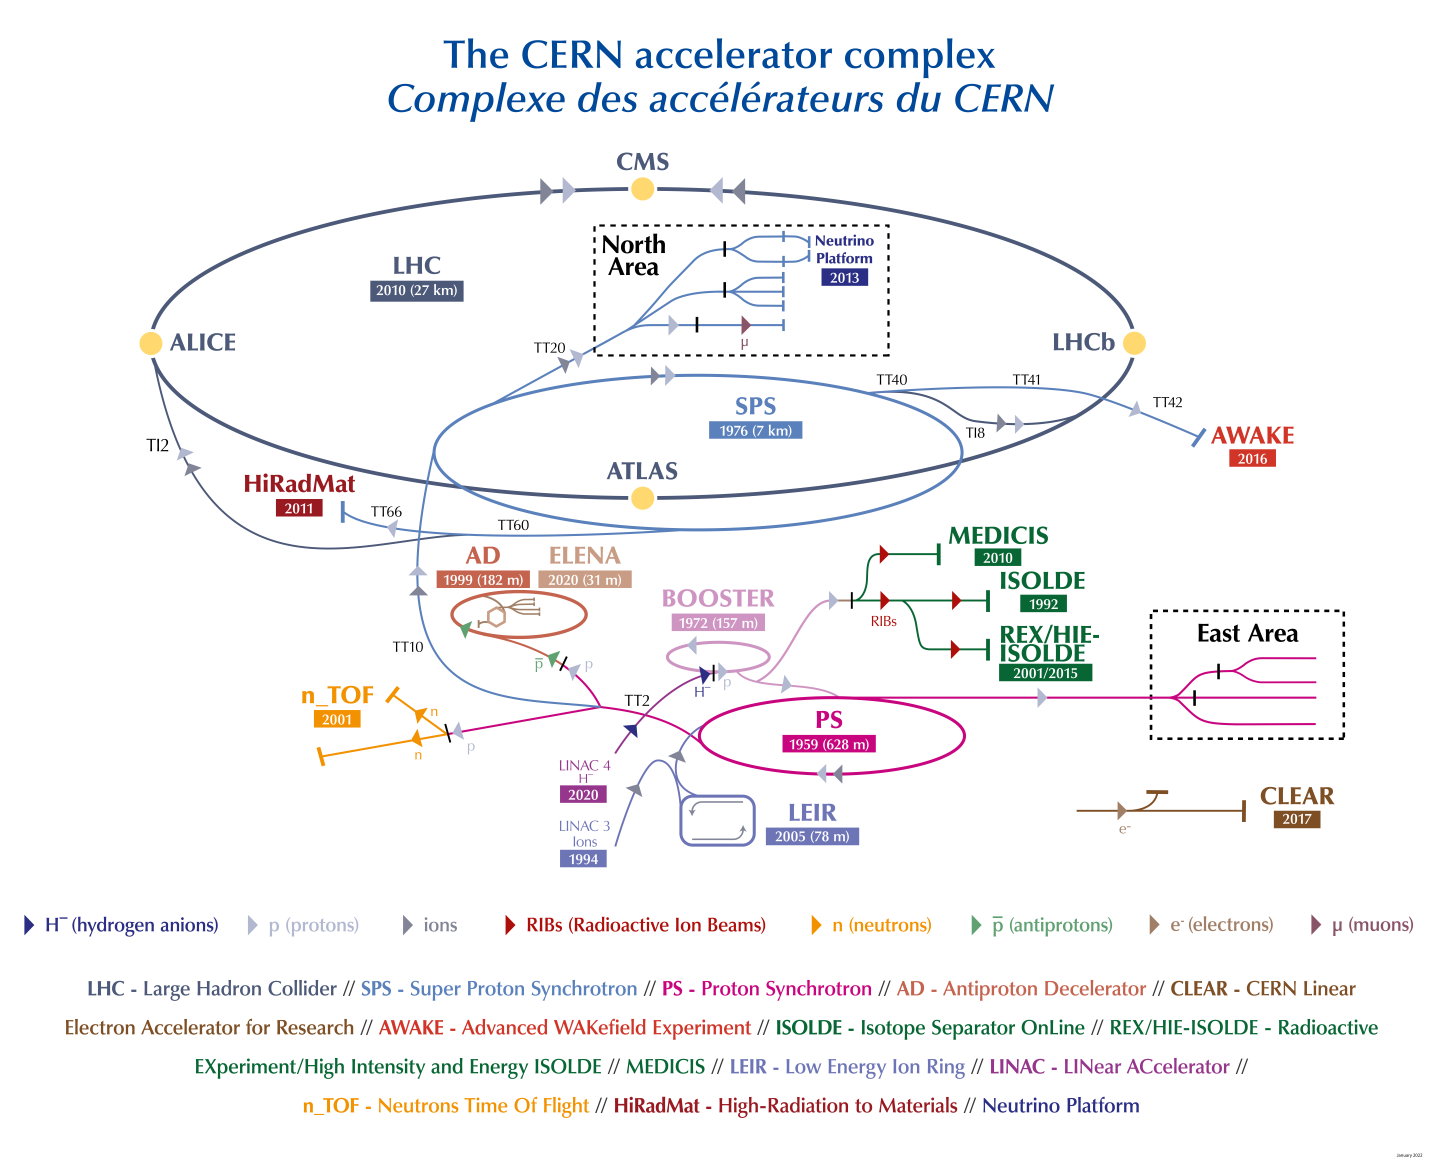
\includegraphics[width=1\textwidth]{images/introduction/cern_accelerator_complex.png}
        \caption{Schematic view of the CERN accelerator complex. The different colors correspond to the different machines. The year of commissioning and the type of particles used in each one of them are also indicated along with the circumference for the circular machines. The image is a courtesy of CERN.}
        \label{fig:cern_accelerator_complex}
 \end{figure}

 It is worth mentioning that not only protons but also led ions are accelerated in the LHC, starting their journey from Linac3 and LEIR and then following the same route with proton beams.


 Last, the accelerators in the injector chain not only prepare the beam for the LHC but also provide beams to various other facilities and experiments at lower energies. Examples are the Anti-proton Decelerator (AD) which studies the antimatter, the Online Isotope Mass Separator (ISOLDE) which studies the properties of the atomic nuclei using radioactive beams, and the Advanced Proton Driven Plasma Wakefield Acceleration Experiment (AWAKE) which investigates the particles' acceleration by proton-driven plasma wakefield.

 \subsection{The CERN Super Proton Synchrotron}
 % sps history: https://be-dep-op-sps.web.cern.ch/history
 The majority of the research described in this thesis was conducted for the Super Proton Synchrotron (SPS). Thus, some additional information about this machine is provided here. The SPS (shown with light blue color in Fig.~\ref{fig:cern_accelerator_complex}) was switched on in 1967 and has a circumference of 6.9\,km. It used to operate as a proton-antiproton collider ($\mathrm{Sp\bar{p}S}$) and later on as an injector for the Large Electron Positron collider (LEP) while it also provided beams for fixed-target experiments (e.g. in the North Area). Even though the SPS can accelerate various particle types (protons, antiprotons, electrons, and heavy ions) the following information will concern its operation with proton beams which is the topic of the research presented in this thesis.

 Currently, the SPS is the second biggest accelerator at CERN and it can accelerate protons in from 26\,GeV up to 450\,GeV. Due to its past use as a collider, it can also operate as a storage ring. This operational mode is called "coast" and was used for the majority of the experimental studies presented in this thesis. During coast, the bunches circulate in the machine for long periods at constant energy. The highest energy at which SPS can operate in coast is 270\,GeV. 

 %After that they are injected in the LHC. Hoewever, as it used to be a collider it can operate as a storage ring, it is called coast (des ti exeis grapsei.) and will be used for the studies in this thesis.
 



\section{High-Luminosity LHC project and Crab Cavities}
%LHC is the flagship of the CERN accelerator complex and is the at the cutting edge of the accelerator and high energy physics research with almost ten thousand scientists working for and with it. In order to extend its discovery potential LHC will undergo a major upgrade in the coming years. 
% Hl-lhc book: p.2 hl-lhc is the top priority of the european strategy of particle physics. 
High-Luminosity LHC (HL-LHC)~\cite{HL_LHC_yellow_report, Brning2015} is the upgrade of the LHC machine which will extend its potential for discoveries. In particular, it aims to increase its instantaneous luminosity by a factor of 5 beyond the current operational values and the integrated luminosity by a factor of 10. 

The luminosity, along with the energy, is a key parameter defining the performance of a collider as it is a measure of the collisions rate. The instantaneous luminosity is expressed as~\cite{luminosity}:

\begin{equation}\label{eq:luminosity_inst}
    \mathcal{L} = \frac{n_b f_\mathrm{rev}N_1 N_2}{4 \pi \sigma_x \sigma_y} \frac{1}{\sqrt{1+(\frac{\sigma_z}{\sigma_\mathrm{xing}} \frac{\theta_c}{2})^2}},
\end{equation}

where $\frev$ is the revolution freuency of the machine, $n_b$ is the number of colliding bunch pairs, $N_{1,2}$ is the bunch intensity, $\sigma_{x,y}$ is the transverse beam size at the interaction point, $\sigma_z$ the rms bunch length, $\sigma_{\mathrm{xing}}$ the transverse beam size in the crossing plane and $\theta_c$ is the full crossing angle between the colliding beams. The crossing angle, is often introduced between the bunches in a collider to reduce parasitic collisions and get rid of the remenants after the collision. For reference, in the LHC machine, the crossing angle is in the order of magnitude $\mathrm{\mathrm{\mu rads}}$.


The integrated luminosity, is the one that ultimately defines the performance of the machine as it provides the total number of recorderd events. It depends both on the instantaneous luminosty and on the machine availability. The integrated luminosity, is expressed as~\cite{HL_LHC_yellow_report}:
\begin{equation}\label{eq:integrated_luminosity}
    \mathcal{L}_I \equiv \int_{\Delta t} \mathcal{L} dt,
\end{equation}

where $\mathcal{L}$ is the instantaneous luminosity as defined in Eq.~\eqref{eq:luminosity_inst}.
% for more details and specific values check sofias thesis.
% and: https://accelconf.web.cern.ch/ipac2015/papers/thxb2.pdf

HL-LHC aims to achive instantaneous luminosity of $\mathcal{L} \sim 5 \cdot 10^{34} \ \mathrm{cm^{-2} s^{-1}}$ and an increase on the integrated luminosity from 300 $\mathrm{fb^{-1}}$ to 3000 $\mathrm{fb^{-1}}$. % Source: https://accelconf.web.cern.ch/ipac2019/papers/mopgw095.pdf

%\normalsize{\textbf{Crab Cavities}}\\
\subsection{Crab Cavities}\label{subsec:CC_intro}
To achieve its luminosity goals, HL-LHC will employ numerous innovative technologies. Crab Cavity technology (will be denoted as $\CC$ in this thesis)~\cite{Calaga:2673544} is one of the key componenets of the project as it will be employed to restore the luminosity reduction caused by the crossing angle, $\theta_c$ (see Eq.~\eqref{eq:luminosity_inst}).

Crab Cavity is an RF cavity which provides a transverse, sinusoidal like, kick to the particles depending on their longitudinal position within the bunch. A graphic visualisation of the kick is shown in the Fig.~\ref{fig:cc_simple_kick}. It can be seen that the head (leading part) and the tail (trailing part) of the bunch recieve opposite deflection while the particles at the center remain unaffected.

\begin{figure}[!h] % at the directory of ipac22
    \centering         
    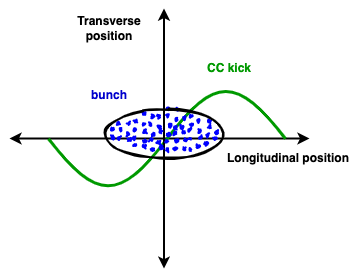
\includegraphics[width=0.5\textwidth]{images/introduction/sin_CC_kick_LHC_beams.drawio.png}
        \caption{Visualisation of the CC kick (green line) on the bunch particles (blue dots). The bunch here appears much smaller than the CC wavelength which means that only the linear part of the kick affects the bunch. This will be the case for the HL-LHC scenario.}
        \label{fig:cc_simple_kick}
 \end{figure}

The $\CC$s will be installed in the two main interaction points of LHC, ATLAS and CMS. According to the plan, four $\CC$s will be installed on each side of the interaction points (two for each ring). This is displayed in Fig.~\ref{fig:LHC_layout_CCs} with the red (ATLAS) and orange (CMS) markers. 

\begin{figure}[!h] % made at diagrams.net saved at google docs
    \centering         
    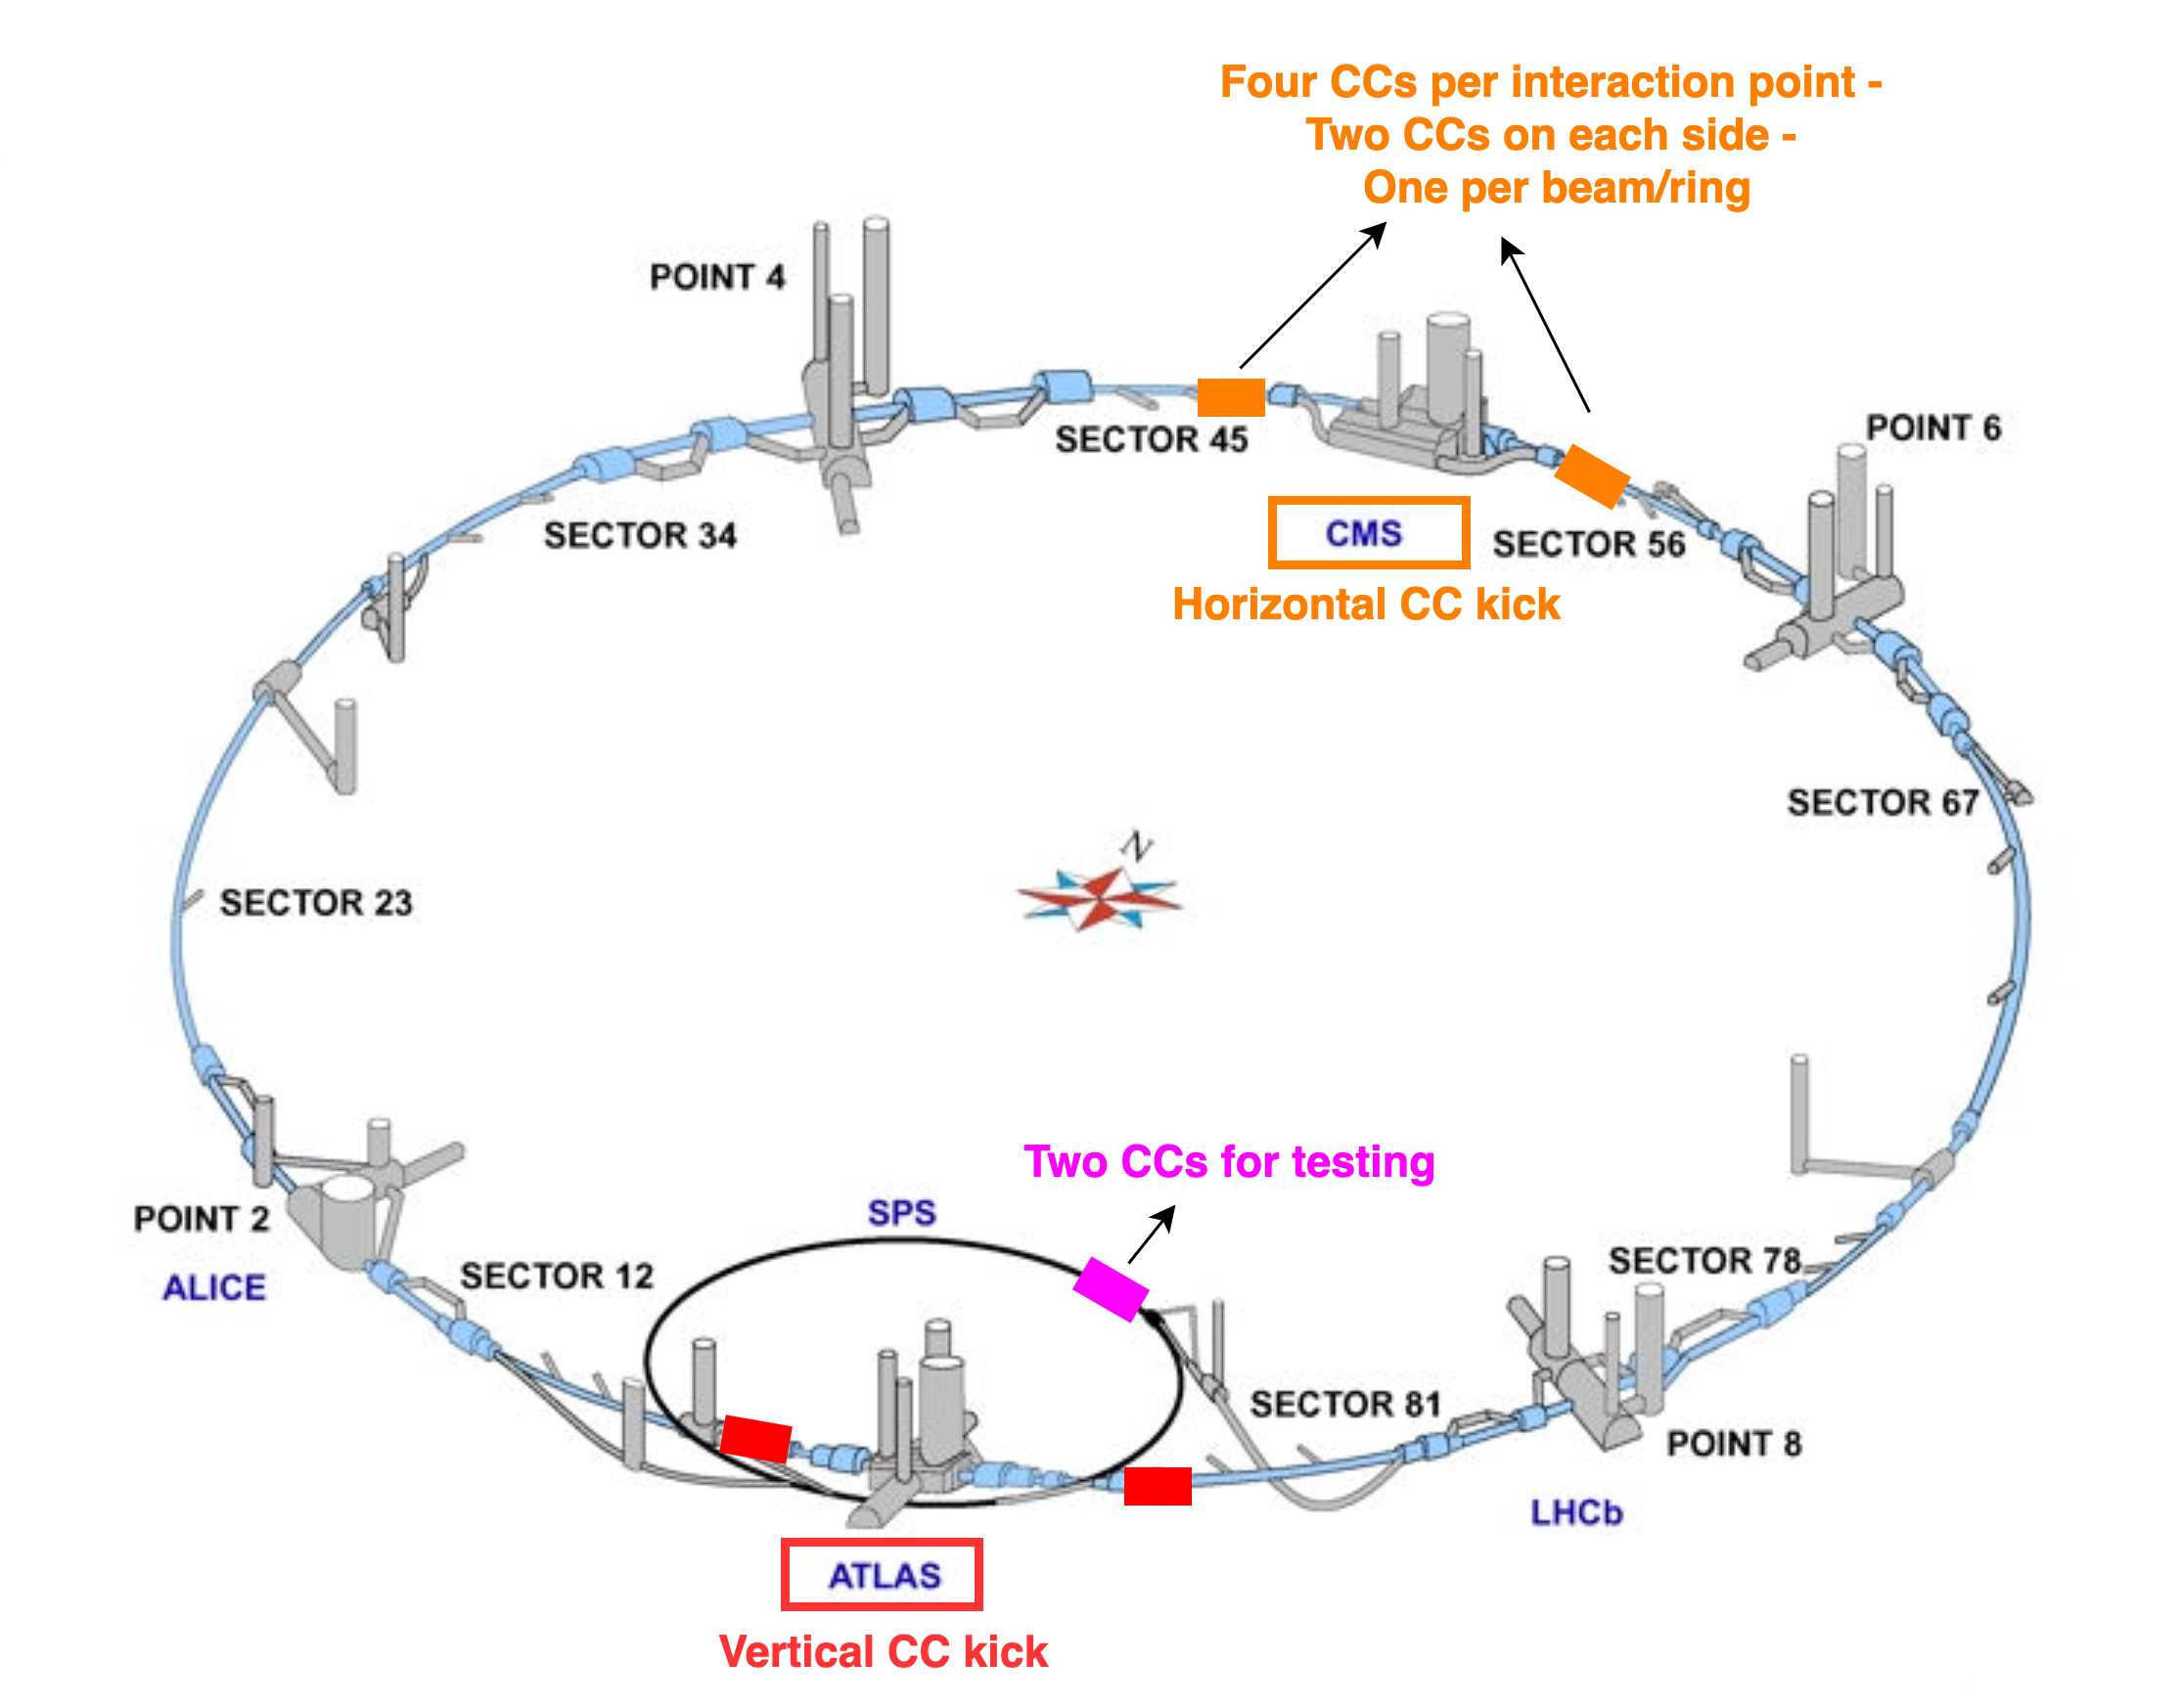
\includegraphics[width=0.8\textwidth]{images/introduction/LHC_layout_CCs.png}
        \caption{Layout of the LHC and the SPS. The CC location for the HL-LHC configuration is marked. Two CCs (one per ring) will be installed at each side of ATLAS (red) and CMS (orange). Two protoype CCs were also installed in the SPS (magenta) in 2018, to be tested before their installation in LHC. The layout can be found in Ref.~\cite{LHC_SPS_layout} and was modified inspired by Ref.~\cite{LHC_SPS_layout_v2}.}
        \label{fig:LHC_layout_CCs}
 \end{figure}

In this configuration, the bunches recieve the transverse deflection from the first pair of $\CC$s just before reaching the interaction point. This results to a rotation of the bunch, which mitigates the crossing angle and restores the head-on collisions. The deflection, is cancelled once the bunches reach the second pair of $\CC$s which are symmetrically installed at the opposite side of the interaction point. The collision of the bunches in the presence of the $\CC$s is illustrated in Fig.~\ref{fig:crossing_with_and_without_CCs}~\cite{Verdú-Andrés:2263119}.
% 90 deg between CCs and IP. https://cds.cern.ch/record/2263119/files/10.1016_j.nuclphysbps.2015.09.025.pdf

\begin{figure}[!ht]
    \centering
    \begin{subfigure}[t]{0.45\textwidth}
        \centering
        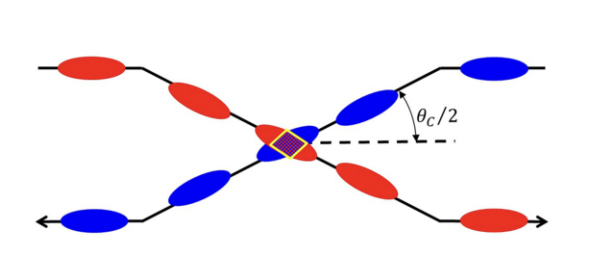
\includegraphics[width=1\textwidth]{images/introduction/no_crab_crossing.png}
        \caption{Crossing without CCs}
        %\label{fig:add_label_here}
    \end{subfigure}
    \hfill
    \begin{subfigure}[t]{0.45\textwidth}
        \centering
        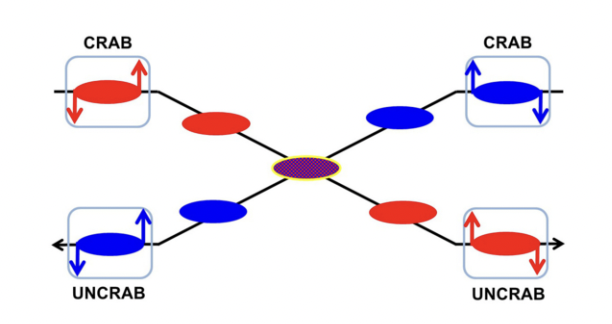
\includegraphics[width=1\textwidth]{images/introduction/crab_crossing.png}
        \caption{Crossing with CCs}
        %\label{fig:add_label_here}
    \end{subfigure}
    \hfill
     \caption{Collision with and without the use of CCs~\cite{Verdú-Andrés:2263119}. CCs restore the overlap between the bunches recovering the luminosity reduction cauased by the crossing angle, $\theta_c$. The blue and red colors indicate the two different bunches.} 
     \label{fig:crossing_with_and_without_CCs}
 \end{figure}


% Local vs global CC scheme: https://slideplayer.com/slide/10896302/ 
The above scheme, with $\CC$s before and after the interaction point, is called the local crabbing scheme. An alternative scheme, named the global crabbing scheme, was also under discussion in the first stages of the project. In such as scheme, the closed orbit distortion that is caused by the fact that the head and the tail of the bunch are kicked in opposite directions propagates in the ring, resulting in transverse bunch oscillations.~\cite{Brning2015}. This scheme is cost-efficient compared to the local scheme as it only requires two CCs. However, it introduces significant constraints on the betatron phase advance between the interaction points and the CCs. The constraints are enhanced by the fact that the bunch crossing in ATLAS takes place in the vertical plane while in CMS in the horizontal. To this end, the local CC scheme was chosen for the HL-LHC configuration. % uncrabbing.
%HL-LHC book p.138: The transverse kick introduced by this cavity, different  for  the  head  and  the  tail  of  each  bunch,  is  equivalent  to  a  closed  orbit  distortion, i.e. head and tail would follow their individual closed orbit around the ring, their tilt wobbling around the unperturbed closed orbit of the bunch center.

% short summary about KEKB in sylivias paper: https://cds.cern.ch/record/2263119/files/10.1016_j.nuclphysbps.2015.09.025.pdf
The $\CC$s have been succesfully used in KEKB collider ($e^{+} - e^{-}$) in Japan, during 2007-2010, with lepton beams~\cite{CC_KEKB_4440798, Funakoshi:1955812, oide:pac07-mozaki01}. However, there are significant differences on the beam dynamics in the presence of $\CC$s in lepton and hadron (HL-LHC case) beams. One of the most crucial points, is the impact of errors (e.g. RF noise) which leads in beam degradation~\cite{Calaga:2773279, Alekou:2696109}. For lepton beams, this is not an issue of concern as they nevertheless experience a beam-size damping due to synchrotron radiation. For proton beams the synchrotron radiation damping is much weaker and therefore the beam degradation can lead to emittance growth which eventually can limit the luminosity lifetime.

% other crabbing errors: phase and amplitude rf noise, wakefields (Calaga)
% other difference between letptons and protons (protons: much longer bunches)



1. References to some technical specifications for both CC types. \\

2. Noise, reference to noise studies ... to kek. mention why they are different.\\

3. Reference to kek. CCs have already been used succesfully in KEK in japan with leptons to achieve record luminosity values.\\

4. That's why we need to test them in the SPS. reference more details in ch4
Two main difference, with kekb global scheme and leptons







Concerns about the CCs, noise in their RF system. Wich will results in loss of luminsotiy. mention constraints with references. Luis medina thesis reference.

\section{Motivation, objectives and thesis outline}

